\resizebox{0.4\textwidth}{!}{%
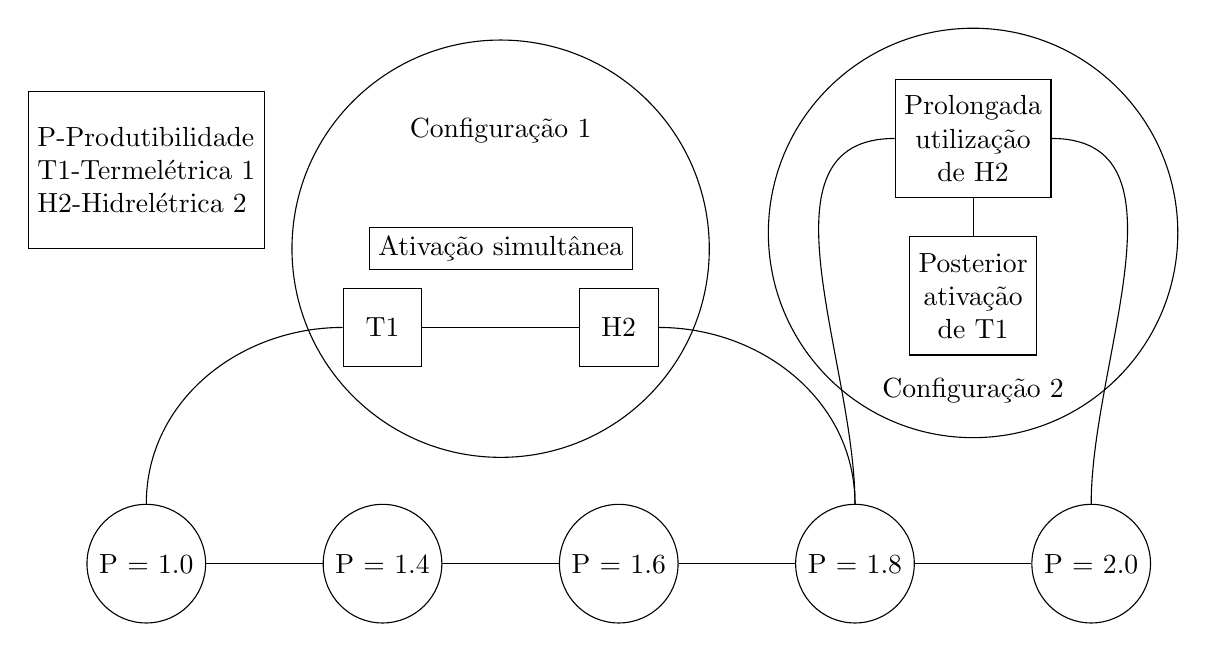
\begin{tikzpicture}
  \draw node[draw, circle] (p10) at (1,1) {P = 1.0};
  \draw node[draw, circle] (p14) at (4,1) {P = 1.4};
  \draw node[draw, circle] (p16) at (7,1) {P = 1.6};
  \draw node[draw, circle] (p18) at (10,1) {P = 1.8};
  \draw node[draw, circle] (p20) at (13,1) {P = 2.0};
  \draw [draw] (p10) to [out=0,in=180] (p14);
  \draw [draw] (p14) to [out=0,in=180] (p16);
  \draw [draw] (p16) to [out=0,in=180] (p18);
  \draw [draw] (p18) to [out=0,in=180] (p20);
  \node [draw](S) at (5.5,5.0) {Ativa\c c\~ao simult\^anea};
  \node [draw, circle, minimum size=5.3cm](c1) at (5.5,5.0) {};
  \node [draw, minimum size=1.0cm] (t1) at (4,4) {T1};
  \node [draw, minimum size=1.0cm] (h2) at (7,4) {H2}; 
  \draw [draw] (t1) to [out=0,in=180] (h2); 
  \draw [draw] (p10) to [out=90,in=180] (t1); 
  \draw [draw] (p18) to [out=90,in=0] (h2); 
  \draw node [] at (5.5, 6.5){Configura\c c\~ao 1};
  \draw node[align=center,draw, minimum size=1.5cm](h) at (11.5,6.4) {Prolongada\\ utiliza\c c\~ao \\de H2};  
  \draw [draw] (p18) to [out=90,in=180] (h);
  \draw [draw] (p20) to [out=90,in=0] (h);
  \draw node[align=center,draw, minimum size=1.5cm](t) at (11.5,4.4) {Posterior\\ ativa\c c\~ao \\de T1};  
  \draw [draw] (h) to [out=270,in=90] (t);
  \node [draw, circle, minimum size=5.2cm](c1) at (11.5,5.2) {};
  \draw node [] at (11.5, 3.2){Configura\c c\~ao 2};
  \node [draw,align=justify, minimum size=2cm]() at (1.0,6.0) {P-Produtibilidade\\
  T1-Termel\'etrica 1\\H2-Hidrel\'etrica 2 };
\end{tikzpicture}}
